\documentclass[]{llncs}

\usepackage{amsmath}
\usepackage{graphicx}
\usepackage{float}
\usepackage{color, colortbl}
\usepackage{xcolor}
\usepackage{caption}
\usepackage{subcaption}

\renewcommand{\labelenumi}{\arabic{enumi}.}
\renewcommand{\labelenumii}{\arabic{enumi}.\alph{enumii})}

\begin{document}

\title{Collision-Free WLANs: From Concepts to Working Protocols. A PhD. Proposal}
\author{Luis Sanabria-Russo}
\institute{Universitat Pompeu Fabra, Barcelona Spain \\ \email{luis.sanabria@upf.edu}}
\maketitle

\begin{abstract}
In the upcoming years the number of devices that exchange data wirelessly is though to increase dramatically, even nowadays home environments no longer lack the wireless network congestion only seen before at office/public spaces (like wireless hot-spots). The current Medium Access Control (MAC) protocol is known to be prone to collisions, which increase with the number of stations in the wireless network. Many proposals have been made to amend the current standard, but at the time of this writing the drawbacks related to collisions have not been fixed. One of the reasons why implementing new MAC protocols is a challenging task relates to the prototyping difficulties associated to the really fast processing speed required to execute the protocol in real-time. Prototype implementations would make it possible to test proposed MAC protocols in realistic channel conditions and traffic patterns.

% to the need for really fast processing speed (which can only be achieved at hardware level) and the need for more realistic channel conditions and traffic scenarios.

This PhD Thesis Proposal aims at designing and prototyping next-generation MAC protocols for IEEE 802.11-like networks, going from concept proposals to hardware implementation.

% These challenges reveal the need for collision-free medium access control protocols capable of allocating large number of stations that are foreseeable in the future of wireless local area networks. Furt


% The current standard for medium access control in Wireless Local Area Networks (WLANs) called Carrier Sense Multiple Access with Collision Avoidance (CSMA/CA), is by its nature prone to collisions. These happen as a consequence of randomizing the backoff counter each contender must select in order to coordinate its transmissions. Carrier Sense Multiple Access with Enhanced Collision Avoidance (CSMA/ECA) introduces minor adjustments to CSMA/CA  that eliminate the possibility of collisions after a short convergence period. Its principle is to select a deterministic backoff after successful transmissions instead of a random one (as in CSMA/CA), allowing contenders to \emph{own} a time slot in the schedule. 
\end{abstract}

\section{Introduction}\label{introduction}
	Carrier Sense Multiple Access with Collision Avoidance (CSMA/CA) is the protocol used in wireless local area networks (WLANs) to coordinate transmissions. Nodes should avoid simultaneous transmissions because the medium is shared, so concurrent transmissions attempts will result in indecipherable messages to the receivers. This event is referred to as a \emph{collision}. 

For CSMA/CA, time is slotted. As a result, there are three kind of slots: \emph{empty}, \emph{successful} and \emph{colllision} slots, where successful and collision slots contain succesful transmissions or collision events. While the remaining are just tiny empty slots of a fixed time length.

Every time there is a contend for transmission, CSMA/CA forces contenders to count down from a randomly generated number (from now on referred to as backoff counter), decrementing it by one per every passing empty slot. When the backoff expires (reaches zero), contenders will attempt transmission. Nevertheless, because the backoff counter is generated at random, there might be cases where two o more contenders simultaneuously attempt transmission and a collision occurs, significantly degrading the throughput of the system as more nodes join the contend for the medium.

The focus of this paper is to describe how it is possible to obtain greater levels of throughput than the achieved by CSMA/CA under optimal parameter configuration, by means of picking a deterministic backoff counter after successful transmissions. This approach is called Carrier Sense Multiple Access with Enhanced Collision Avoidance (CSMA/ECA)~\cite{CSMA_ECA}. Results also show that by making this simple modification on the behavior of CSMA/CA, CSMA/ECA preserves the system fairness by equally distributing the system throughput among all contenders. Furthermore, CSMA/ECA is resilient to syncronization flaws on the wireless network cards that can cause a misscount of passing slots (slot drift), as opposed to other MAC protocols~\cite{slotDrift}.

\section{State of the Art}\label{stateOfTheArt}
	For the following paragraphs, an overview of the state of the art is presented. Ranging from the current standard passing through other proposed protocols to end at the description of CSMA/ECA and the Wireless MAC Processor architecture~\cite{WMP}.

It is worthwhile to note that the words \emph{node}, \emph{contenders} and \emph{stations} my be used interchangeably without any different implication.

\subsection{CSMA/CA: the current standard}
Current WLANs run an instance of CSMA/CA protocol. As briefly mentioned in Section~\ref{introduction}, in this time-slotted networks nodes draw a random backoff timer $B\in[0,CW(k)]$ everytime they have a packet to transmit; where $CW(k)=2^{k}CW_{\min}$ is the contention window at backoff stage $k\in[0,m]$ with $m$ its maximum value, and $CW_{\min}$ being the minimum contention window.

Every passing empty slot decrements the backoff counter in one, and freezes when another node's transmission is detected. When the backoff expires ($B=0$), the contending node attempts transmission.

Because the backoff is computed at random, it is possible that two or more nodes pick the same value. When the corresponding stations attempt transmission none will receive an \emph{ACKnowledgement} (ACK) from the receiver, so transmitters assume that the transmission resulted in a collision.

The ways CSMA/CA handles collisions is summarized in the following bullets:
\section{Research Objectives}\label{objectives}
	As was mentioned in the previous sections, CSMA/ECA is capable of achieving higher throughput than CSMA/CA in most common scenarios. Its backoff strategy allows nodes to achieve a collision-free state even for a very large number of CSMA/ECA contenders; while its fairness mechanisms ensure that all stations share the same available system throughput in the long-term.

The following paragraphs detail the general and specific objectives of this research. 

\subsection{General Objective}
In Section~\ref{motivation} is stated that the goal of this PhD Thesis is twofold. Nevertheless, its sole general objective can be described as to:
\begin{itemize}
	\item Design and implement in real hardware a totally distributed collision-free MAC protocol for 802.11-like networks, capable of allocating the high number of contenders expected to be seen in upcoming Small-Office/Home-Office (SOHO) scenarios and ensuring greater levels of throughput than the current standard.
\end{itemize}

\subsection{Specific Objectives}
Ranging from research challenges to debugging, the following subsection details what are believed to be the required steps to accomplish this research's general objective. Each specific objective is composed of \emph{phases} that dictate the activities required to fulfill it.
\begin{enumerate}
	\item Compare CSMA/CA performance with CSMA/ECA by means of simulation.\\
	
	{\bfseries Phases:}
	\begin{enumerate}
		\item Replicate CSMA/CA's behavior in a discrete event-based simulator.\label{buildSimulator}
		\item Progressively incorporate CSMA/ECA features.\label{incorporateECA}
		\item Identify the performance metrics that will allow an unbiased comparison between the two protocols.\label{metrics}
		\item Perform simulation tests for metrics gathering under saturated and unsaturated scenarios\label{scenarios}.
		\item Construct a mixed scenario, where some nodes run CSMA/CA while of others use CSMA/ECA. Repeat the simulations as in Phase~\ref{scenarios}.
		\item Document the results for future comparison with the hardware implementation.\label{simulationResults}\\
	\end{enumerate}
	
	\item Flash WNICs with the default WMP-CSMA/CA protocol to gather data that will work as a control in future testbeds.\label{learningWMP}\\
	
	{\bfseries Phases:}
	\begin{enumerate}
		\item Install the WMP-Editor on a host PC to study its components and configuration.
		\item Identify the required modifications (if any) to replicate CSMA/CA as a WMP.
		\item Develop automated metric gatherings scripts on the client PCs based on those identified in Phase~\ref{metrics}.
		\item Flash the necessary WNICs to replicate ad-hoc and Basic Service Set (BSS) WLANs running WMP-CSMA/CA.
		\item Run experiments with the same parameters used in Phase~\ref{scenarios} and compare the performance evaluation with those obtained in Phase~\ref{simulationResults}.\label{WMPExperiment}\\
	\end{enumerate}

	\item Progressively modify CSMA/CA into CSMA/ECA using WMP and necessary assembly code.\label{ECAinWMP}\\
	
	{\bfseries Phases:}
	\begin{enumerate}
		\item Draw an example of CSMA/ECA using WMP-Editor in order to identify the required modifications.\label{WMPModifications}
		\item Access the underlying ByteCode and identify the segments that correspond with Phase~\ref{WMPModifications}\label{accessByteCode}.
		\item Design or modify the necessary XFSM that would allow the translation of CSMA/ECA into a WMP.
		\item Flash WNICs with the CSMA/ECA protocol and repeat the experiments as performed in Phase~\ref{WMPExperiment}.\\
	\end{enumerate}

	\item Extend the functionality of CSMA/ECA to RFID in the attempt of reducing the convergence and tag-reading time.\label{ECAinRFID}\\
	
	{\bfseries Phases:}
	\begin{enumerate}
		\item Gather metrics about the current performance of the system.
		\item Adapt CSMA/ECA to replace current MAC protocol.
		\item Design a simulation environment where metrics can be gathered so a performance evaluation can be made. 
		\item Document the results and compare them with the performance of the network before incorporating CSMA/ECA.\\
	\end{enumerate}

\end{enumerate}

\section{Research Plan and Methodology}\label{planAndMethod}
	In order to fulfill the objectives described in Section~\ref{objectives}, a convenient and dynamic methodology should be implemented.

Given the great deal of software development, reverse engineering and debugging involved in the specific objectives, it is required to build a research plan with a methodology able to: 
\begin{itemize}
	\item Adapt to constant changes in the specific objectives/phases, even at advanced stages.
	\item Consider collaboration with peers acquainted with other knowledge areas.
	\item Facilitate frequent working-software deliveries with minimum bugs.
\end{itemize}

Based on this, it is thought to implement the principles of Agile Software Development~\cite{agileAlliance,agileManifesto}, which very well correspond with the requirements mentioned above.

\subsection{Shot-term Control}\label{shot-termContol}
Following the recommendations provided by the Agile methodology, a fifteen-minute meeting will be held everyday (if possible) with the thesis supervisor. This short, and preferably standing-up meetings complement the process of development by:

\begin{itemize}
	\item Keeping everyone up-to-date on the state of the development.
	\item Increases supervisor-student collaboration.
	\item Helps keep the high frequency of the technical reports.
\end{itemize}

These technical reports must provide a sufficient overview of the research efforts, including:

\begin{itemize}
	\item Current state of the research (looking at the objectives/phases).
	\item Past, current and future tasks (up until the next report).
	\item Required knowledge or material to fulfill the current objective/phases.
\end{itemize}

By implementing the Agile recommendations and following the short-term control measures described above, it is possible to keep track of the efforts towards the general objective.

\subsection{Description of the Plan by Years}
Agile methods are thought to be adaptive, meaning that the far future (six months from now) will present unknown problems; nevertheless it is more efficient at solving short-term problems, as was described previously at Section~\ref{shot-termContol}.

To leverage this issue, the objectives presented in Section~\ref{objectives} can be distributed in the remaining years as follows:

\begin{itemize}
	\item {\bfseries First year:} at the time of this writing, objectives~\ref{buildSimulator},~\ref{incorporateECA},~\ref{metrics},~\ref{scenarios} are at their final phase. Further details can encountered at Section~\ref{priorWork}. The remaining phases of the first specific objective are to be finished during the first year.
	\item {\bfseries Second year:} will be dedicated to the study of the WMP architecture. This step will provide the knowledge to continue achieving objectives. It is expected to achieve specific objective~\ref{learningWMP}, as well as~\ref{WMPModifications} and~\ref{accessByteCode}.
	\item {\bfseries Third year:} is to be dedicated at the completion of specific objective~\ref{ECAinWMP} and~\ref{ECAinRFID}.
\end{itemize}

A summary of the distribution of the activities throughout the remaining years is shown in Figure~\ref{fig:gantt}.

\begin{figure}[htbp]
  \centering
  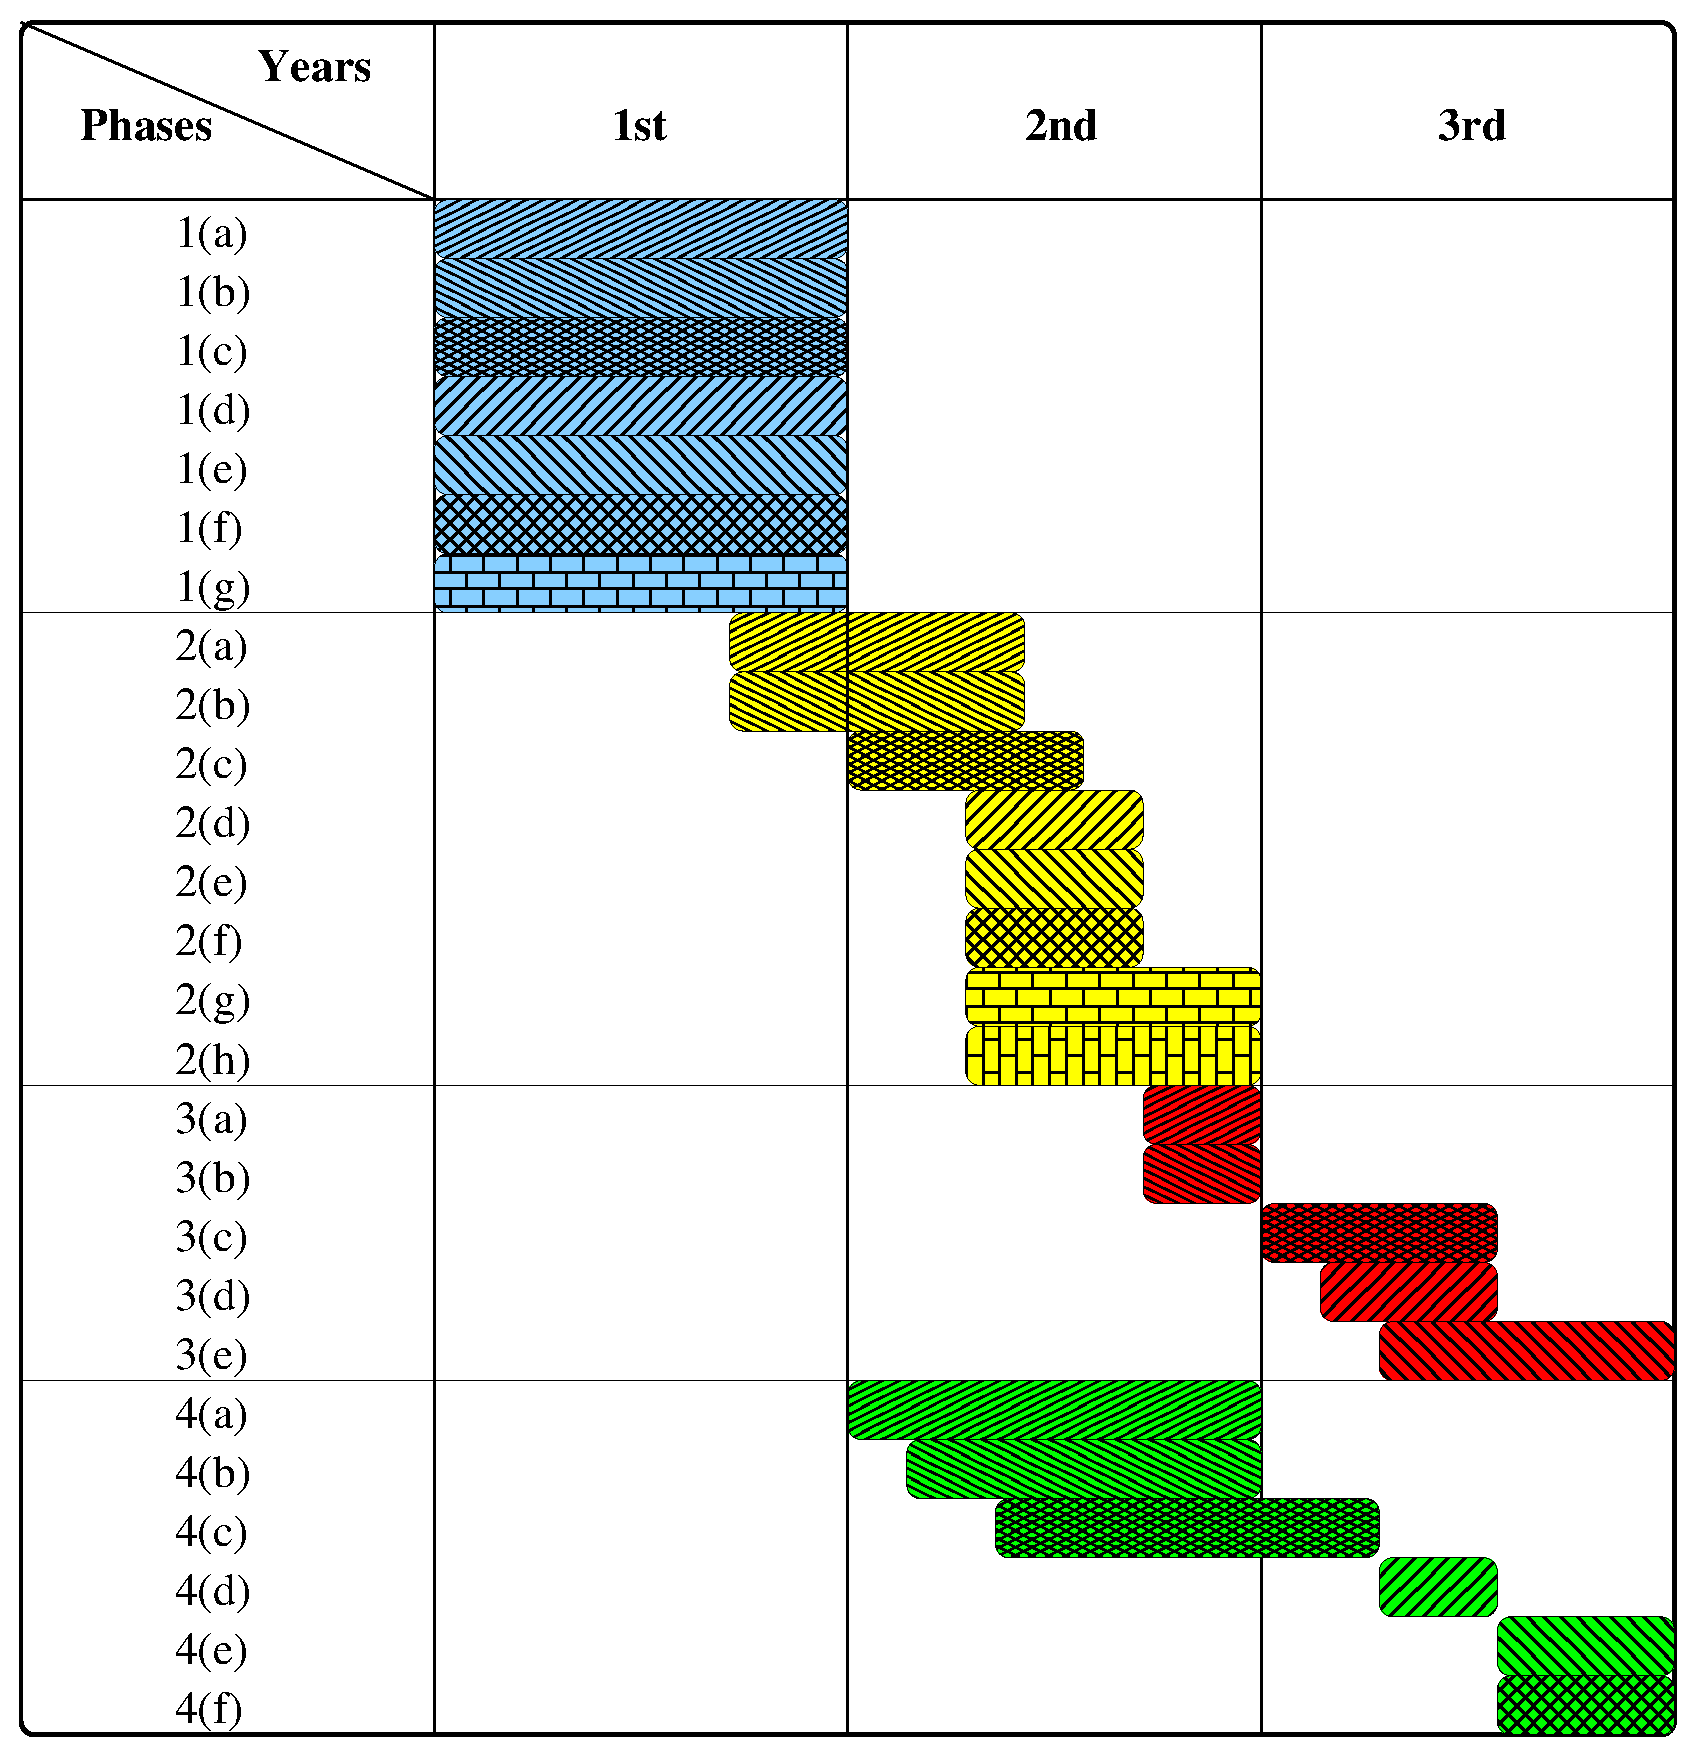
\includegraphics[width=0.9\linewidth]{gantt.eps}
  \caption{Gantt diagram
  \label{fig:gantt}}
\end{figure}
\section{Summary of Prior Work}\label{priorWork}
	As was mentioned in Section~\ref{planByYears}, most of the first specific objective has been successfully developed. Its results derived in collaboration with experts from international institutions and two publications:

\begin{enumerate}
	\item Sanabria-Russo, L., Barcelo, J., Bellalta, B: ``Fairness in Collision-Free WLANs''. INFOCOM 2013 Student Poster Session, Turin - Italy. ArXiv e-prints (February 2013).\label{posterInfocom}
	\item Sanabria-Russo, L., Faridi, A., Bellalta, B., Barcelo, J., Oliver, M.: ``Future Evolution of CSMA Protocols for the IEEE 802.11 Standard''. Second IEEE ICC Workshop on Telecommunications Standards: From Research to Standards (June 2013).\label{ICCPaper}
\end{enumerate}

Results of publication~\ref{posterInfocom}~\cite{fairness-ECA} are summarized in Figure~\ref{fig:INFOCOMPoster}. The work includes the introduction of the concept of hysteresis and fair share to CSMA/ECA. It involved the programming of the MAC protocol in a modified version of the COST simulator~\cite{COST} as well as fruitful collaboration with current members of the team that originally proposed the idea in~\cite{L_MAC2}.\\

Results from publication~\ref{ICCPaper}~\cite{research2standards} are contained in Figure~\ref{fig:ICCPaper}. Apart from showing the throughput enhancements over CSMA/CA, it is also shown how the proportion of collision slots reduces to zero when using CSMA/ECA. Furthermore, code snippets are presented to highlight the slight variations between CSMA/ECA and CSMA/CA.

\begin{figure}[htbp]
\centering
\begin{subfigure}{.5\textwidth}
  \centering
  \includegraphics[width=\linewidth]{ECA-vs-CA-FINAL.eps}
  \caption{(a)}
  \label{fig:DCFvsECA}
\end{subfigure}%
\begin{subfigure}{.5\textwidth}
  \centering
  \includegraphics[width=\linewidth]{ECA-w-enhancements-FINAL.eps}
  \caption{(b)}
  \label{fig:ECAPerformace}
\end{subfigure}
\caption{\ref{fig:DCFvsECA}) Throughput of CSMA/CA vs. CSMA/ECA without hysteresis and fair share. \ref{fig:ECAPerformace}) Throughput and fairness when incorporating hysteresis and fair share to CSMA/ECA.}
\label{fig:INFOCOMPoster}
\end{figure}

\begin{figure}[htbp]
\centering
\begin{subfigure}{.5\textwidth}
  \centering
  \includegraphics[width=0.7\linewidth,angle=-90]{avgCollisions-12sta.eps}
  \caption{(a)}
  \label{fig:avgCollisions}
\end{subfigure}%
\begin{subfigure}{.5\textwidth}
  \centering
  \includegraphics[width=0.7\linewidth,angle=-90]{throughput-combined.eps}
  \caption{(b)}
  \label{fig:throughputCombined}
\end{subfigure}
\caption{\ref{fig:avgCollisions}) Cumulative fraction of slots spent in collisions for $N=12$ nodes. \ref{fig:throughputCombined}) Throughput.}
\label{fig:ICCPaper}
\end{figure}


\section{Significance}\label{significance}
	It is not hard to encounter the crowded WLANs scenario exemplified in Section~\ref{motivation}. Even nowadays it is not rare to have multiple WiFi devices at home attempting to access the channel at the same time: watching an on-line video stream, surfing the Web, receiving VoIP calls and uploading data from your personal health monitoring device.

CSMA/CA has been the de facto standard for coordinating transmissions in WLANs; nevertheless, its performance degrades when imposing heavy traffic on crowded scenarios like the one proposed above, where tens of devices must coordinate their transmission attempts in a totally distributed manner. This degradation in the system performance can be appreciated in the form of video lags while streaming or in below-average download speeds.

By removing the randomness from the contention mechanism of CSMA/CA, CSMA/ECA achieves a better performance while allowing many nodes to coexist in a collision-free environment. Nevertheless, CSMA/ECA lacks a thorough study of the different scenarios that it could face regarding: Quality of Service (QoS), hidden/exposed node mechanisms, performance against different traffic patterns and contention parameters optimization; which on the other hand have been the focus of study in CSMA/CA for many years.

Although it has proven to best CSMA/CA's throughput in controlled simulation environments, CSMA/ECA is far away from being considered as an amend to the standard.

This work aims at bringing the benefits of CSMA/ECA to home WLANs. 

\bibliographystyle{splncs}
\bibliography{ref}

\end{document}

